\input{preamble.tex}
\usepackage{eurosym} % pour le symbole euro propre

\begin{document}

\reversemarginpar

\pagestyle{fancy}
\fancyhead[L]{Terminale STMG}
\fancyhead[C]{\textbf{DS n°5 - Fonction inverse et polynômes - 2a}}
\fancyhead[R]{\today}

\null\vspace{-30pt}
Nom / Prénom : \\

Consignes particulières : 
\begin{itemize}[label=$\bullet$]
	\item 
	La calculatrice est {autorisée}.
	\item 
	L'exercice \ref{exe:1a} peut être fait entièrement sur la feuille.
	\item 
	Toute trace de recherche est prise en compte.
\end{itemize}

\hrule

\exe{5}{

}{exe:1a}{

}

\exe{5}{
On considère la fonction $f$ définie sur $\R$ par $f(x) = x^3 + \frac92 x^2 -12x +8$.
\begin{enumerate}
\item Déterminer la fonction dérivée de $f$ sur $\R$.
\item Montrer que l'on peut écrire :
\[ f'(x) = 3(x-1)(x+4) \]
\item En déduire les valeurs $x$ pour lesquels $f'(x)=0$.
\item Dresser le tableau de variation de $f$ sur $\R$.
\end{enumerate}
}{exe:2a}{
\begin{enumerate}
\item $f'(x) = 3x^2+9x-12$
\item Il suffit de développer l'expression donnée.
\item $x=-4$ et $x=1$.
\item 
\begin{center}
\begin{tikzpicture}
   \tkzTabInit{$x$ / 1 , $f'(x)$ / 1, $f(x)$ / 1.5}{$-\infty$, $-4$, $1$, $\infty$}
   \tkzTabLine{, +, z, -, z, +, }
   \tkzTabVar{ -/ $-\infty$, +/ , -/, +/ $+\infty$ }
\end{tikzpicture}
\end{center}
\end{enumerate}
}

\exe{5}{
On considère la fonction $g$ définie sur $\Ret$ par $g(x) = 4x +7 + \frac{64}{x}$.
\begin{enumerate}
\item Déterminer la fonction dérivée de $g$ sur $\Ret$.
\item Montrer que l'on peut écrire :
\[ g'(x) = \dfrac{4(x-4)(x+4)}{x^2} \]
\item En déduire les valeurs $x$ pour lesquels $g'(x)=0$.
\item Etudier les limites éventuelles de $g$ sur son ensemble de définition.
\item Dresser le tableau de variation de $g$ sur $\Ret$.
\end{enumerate}
}{exe:3a}{
\begin{enumerate}
\item $g'(x)=4-\frac{64}{x^2}$
\item Il suffit de développer.
\item $x=-4$ ou $x=4$
\item On trouve :
\begin{align*}
\lim_{x \to - \infty} g(x) & = - \infty & \lim_{x \to + \infty} g(x) & = + \infty \\
\lim_{\substack{x \to 0 \\ x <0 }} g(x) & = - \infty & \lim_{\substack{x \to 0 \\ x >0 }} g(x) & = + \infty
\end{align*}
\item
\begin{center}
\begin{tikzpicture}
   \tkzTabInit{$x$ / 1 , $f'(x)$ / 1, $f(x)$ / 1.5}{$-\infty$, $-4$, $0$, $4$, $+\infty$}
   \tkzTabLine{, +, z, -, d, -, z, +, }
   \tkzTabVar{-/ $-\infty$ , +/, -D+/ $-\infty$ / $+\infty$, -/, +/ $+\infty$ }
\end{tikzpicture}
\end{center}
\end{enumerate}
}

\exe{5}{
Une entreprise produit des composants électroniques. Le nombre de ces composants fabriqués et vendus est compris entre 100 et 400. 
Le bénéfice réalisé par l'entreprise, exprimé en milliers d'euros, est modélisé par la fonction $f$ définie sur [1 ; 4] par :
\[ \begin{array}{c c c c}
f : & \R & \to & \R \\
& x & \mapsto & -2x^3 + 3x^2+12x-15 \end{array} \]
où la variable $x$ correspond à la centaine de composants fabriqués et vendus.
\begin{enumerate}
\item En considérant la production de l'entreprise, donner les valeurs possibles pour la variable $x$.
Exprimer la réponse sous forme d'un intervalle.
\item Déterminer la dérivée de la fonction $f$.
\item Montrer que l'on peut écrire :
\[ f'(x) = -6(x+1)(x-2) . \]
\item Dresser le tableau de variation de $f$. Restreindre ce tableau aux valeurs de $x$ cohérentes avec la production de l'entreprise.
\item Quel est le nombre de composants fabriqués et vendus qui permet de réaliser le bénéfice maximal ? 
Quel est ce bénéfice maximal ?
\end{enumerate}
}{exe:4a}{
\begin{enumerate}
\item $x \in [1 ; 4]$.
\item $f'(x) = -6x^2 +6x +12$.
\item $-6(x+1)(x-2) = -6(x^2-x-2) = -6x^2 +6x +12$.
\item 
\begin{center}
\begin{tikzpicture}
   \tkzTabInit{$x$ / 1 , $f'(x)$ / 1, $f(x)$ / 1.5}{$1$, $2$, $4$}
   \tkzTabLine{, -, z, +,}
   \tkzTabVar{-/ , +/, -/ }
\end{tikzpicture}
\end{center}
\item La fonction atteint un minimum sur [1 ; 4] en $x=2$ (donc 200 composants) et $f(2)=5$, 
soit un bénéfice maximal de 5~000 \euro.
\end{enumerate}
}

%%%%%%%%%%%%

\setcounter{Exercise}{0}

\newpage

\pagestyle{fancy}
\fancyhead[L]{Terminale STMG}
\fancyhead[C]{\textbf{DS n°5 - Fonction inverse et polynômes - 2b}}
\fancyhead[R]{\today}

\null\vspace{-30pt}
Nom / Prénom : \\

Consignes particulières : 
\begin{itemize}[label=$\bullet$]
	\item 
	La calculatrice est {autorisée}.
	\item 
	L'exercice \ref{exe:1b} peut être fait entièrement sur la feuille.
	\item 
	Toute trace de recherche est prise en compte.
\end{itemize}

\hrule

\exe{5}{
Compléter les phrases suivantes :
\begin{enumerate}[itemsep=6pt]
\item L'inverse de $\dfrac34$ est $\dots$
\item $\lim\limits_{x \to + \infty} \dfrac1{x} = \dots$
\item $\lim\limits_{\substack{x \to 0 \\ x >0 }} \dfrac1{x} = \dots$
\item $\lim\limits_{x \to - \infty} 2x + 7 - \dfrac3{x} = \dots$
\item $\lim\limits_{\substack{x \to 0 \\ x < 0 }} 2x + 7 - \dfrac3{x} = \dots$
\end{enumerate}
\textit{Note : attention au signe devant la fonction inverse !}
}{exe:1b}{
\begin{enumerate}[itemsep=6pt]
\item L'inverse de $\dfrac34$ est $\dfrac43$
\item $\lim\limits_{x \to + \infty} \dfrac1{x} = 0$
\item $\lim\limits_{\substack{x \to 0 \\ x >0 }} \dfrac1{x} = +\infty$
\item $\lim\limits_{x \to - \infty} 2x + 7 - \dfrac3{x} = -\infty$
\item $\lim\limits_{\substack{x \to 0 \\ x < 0 }} 2x + 7 - \dfrac3{x} = +\infty$
\end{enumerate}
}

\exe{5}{
On considère la fonction $f$ définie sur $\R$ par $f(x) = -x^3 + 3 x^2 +24x - 9$.
\begin{enumerate}
\item Déterminer la fonction dérivée de $f$ sur $\R$.
\item Montrer que l'on peut écrire :
\[ f'(x) = -3(x-4)(x+2) \]
\item En déduire les valeurs $x$ pour lesquels $f'(x)=0$.
\item Dresser le tableau de variation de $f$ sur $\R$.
\end{enumerate}
}{exe:2b}{
\begin{enumerate}
\item $f'(x) = -3x^2+6x+24$
\item Il suffit de développer l'expression donnée.
\item $x=-2$ et $x=4$.
\item 
\begin{center}
\begin{tikzpicture}
   \tkzTabInit{$x$ / 1 , $f'(x)$ / 1, $f(x)$ / 1.5}{$-\infty$, $-2$, $4$, $\infty$}
   \tkzTabLine{, -, z, +, z, -, }
   \tkzTabVar{ +/ $+\infty$, -/ , +/, -/ $-\infty$ }
\end{tikzpicture}
\end{center}
\end{enumerate}
}

\exe{5}{
On considère la fonction $g$ définie sur $\Ret$ par $g(x) = 5x - 8 + \frac{45}{x}$.
\begin{enumerate}
\item Déterminer la fonction dérivée de $g$ sur $\Ret$.
\item Montrer que l'on peut écrire :
\[ g'(x) = \dfrac{5(x-3)(x+3)}{x^2} \]
\item En déduire les valeurs $x$ pour lesquels $g'(x)=0$.
\item Etudier les limites éventuelles de $g$ sur son ensemble de définition.
\item Dresser le tableau de variation de $g$ sur $\Ret$.
\end{enumerate}
}{exe:3b}{
\begin{enumerate}
\item $g'(x)=5-\frac{45}{x^2}$
\item Il suffit de développer.
\item $x=-3$ ou $x=3$
\item On trouve :
\begin{align*}
\lim_{x \to - \infty} g(x) & = - \infty & \lim_{x \to + \infty} g(x) & = + \infty \\
\lim_{\substack{x \to 0 \\ x <0 }} g(x) & = - \infty & \lim_{\substack{x \to 0 \\ x >0 }} g(x) & = + \infty
\end{align*}
\item
\begin{center}
\begin{tikzpicture}
   \tkzTabInit{$x$ / 1 , $f'(x)$ / 1, $f(x)$ / 1.5}{$-\infty$, $-3$, $0$, $3$, $+\infty$}
   \tkzTabLine{, +, z, -, d, -, z, +, }
   \tkzTabVar{-/ $-\infty$ , +/, -D+/ $-\infty$ / $+\infty$, -/, +/ $+\infty$ }
\end{tikzpicture}
\end{center}
\end{enumerate}
}

\exe{5}{
Une entreprise produit des composants électroniques. Le nombre de ces composants fabriqués et vendus est compris entre 50 et 300. 
Le bénéfice réalisé par l'entreprise, exprimé en milliers d'euros, est modélisé par la fonction $f$ définie sur [0,5 ; 3] par :
\[ \begin{array}{c c c c}
f : & \R & \to & \R \\
& x & \mapsto & -x^3 - 3x^2+9x - 1 \end{array} \]
où la variable $x$ correspond à la centaine de composants fabriqués et vendus.
\begin{enumerate}
\item En considérant la production de l'entreprise, donner les valeurs possibles pour la variable $x$.
Exprimer la réponse sous forme d'un intervalle.
\item Déterminer la dérivée de la fonction $f$.
\item Montrer que l'on peut écrire :
\[ f'(x) = -3(x+3)(x-1) . \]
\item Dresser le tableau de variation de $f$. Restreindre ce tableau aux valeurs de $x$ cohérentes avec la production de l'entreprise.
\item Quel est le nombre de composants fabriqués et vendus qui permet de réaliser le bénéfice maximal ? 
Quel est ce bénéfice maximal ?
\end{enumerate}
}{exe:4b}{
\begin{enumerate}
\item $x \in [0,5 ; 3]$.
\item $f'(x) = -3x^2 -6x +9$.
\item $-3(x+3)(x-1) = -3(x^2+2x-3) = -3x^2 -6x +9$.
\item
\begin{center}
\begin{tikzpicture}
   \tkzTabInit{$x$ / 1 , $f'(x)$ / 1, $f(x)$ / 1.5}{$0.5$, $1$, $3$}
   \tkzTabLine{, -, z, +,}
   \tkzTabVar{-/ , +/, -/ }
\end{tikzpicture}
\end{center}
\item La fonction atteint un minimum sur [0,5 ; 3] en $x=1$ (donc 100 composants) et $f(1)=4$, 
soit un bénéfice maximal de 4~000 \euro.
\end{enumerate}
}

%%%%%%%%%%%%

\newpage
\fancyhead[C]{\textbf{Solutions}}
Les solutions sont données dans l'ordre sujet a puis b. \newline
\shipoutAnswer


\end{document}
